\documentclass[11pt,letterpaper]{article}
\usepackage[margin=0.87in]{geometry}
\usepackage[T1]{fontenc}
\usepackage{lmodern}
\usepackage{microtype}
\usepackage{amsmath}
\usepackage{xcolor}
\usepackage{graphicx}
\usepackage{tikz}
\usepackage{pgfplots}
\pgfplotsset{compat=1.18}
\usetikzlibrary{arrows.meta,calc,positioning,patterns,decorations.pathmorphing,shapes.misc}
\usepackage{booktabs,tabularx,array}
\usepackage{float}
\usepackage{needspace}
\usepackage[font=small,labelfont=bf,labelsep=period,skip=4pt]{caption}
\usepackage{fancyhdr}
\usepackage[colorlinks=true,linkcolor=teal!65!black,urlcolor=teal!65!black,citecolor=teal!65!black]{hyperref}

% Palette (the same as the first paper's plain-language edition)
\definecolor{ink}{HTML}{17324D}
\definecolor{accent}{HTML}{176B70}
\definecolor{pale}{HTML}{EDF5F4}
\definecolor{curl}{HTML}{C8742B}     % the curled arrangement
\definecolor{curlpale}{HTML}{F6E3D3}
\definecolor{flat}{HTML}{2E7D8C}     % the flat arrangement
\definecolor{flatpale}{HTML}{D6ECF0}
\definecolor{melt}{HTML}{8E6C8A}     % too open
\definecolor{meltpale}{HTML}{E9DEE8}
\definecolor{sun}{HTML}{E0A526}
\definecolor{no}{HTML}{B03A2E}
\definecolor{kExact}{HTML}{176B70}
\definecolor{kMeas}{HTML}{2F5F9E}
\definecolor{kPub}{HTML}{5A5A5A}
\definecolor{kOurs}{HTML}{9A5B00}
\definecolor{kClaim}{HTML}{8A2D5A}

\setlength{\parindent}{0pt}
\setlength{\parskip}{0.62em}
\renewcommand{\baselinestretch}{1.08}
\setlength{\headheight}{14pt}
\pagestyle{fancy}
\fancyhf{}
\fancyhead[L]{\small\color{ink}What the change leaves behind}
\fancyhead[R]{\small Plain-language edition}
\fancyfoot[C]{\small\thepage}
\renewcommand{\headrulewidth}{0.3pt}
\hypersetup{pdftitle={What the change leaves behind: the story behind the experiment},pdfauthor={Emily Smith}}

% Chapter opener, sub-heading, take-away box
\newcommand{\chapterpage}[2]{\par\Needspace{16\baselineskip}\vspace{1.4em}{\color{accent}\small\textbf{#1}}\par\vspace{0.2em}{\color{ink}\LARGE\bfseries #2}\par\vspace{0.5em}}
\newcommand{\takeaway}[1]{\par\medskip\noindent\colorbox{pale}{\parbox{\dimexpr\linewidth-2\fboxsep\relax}{\vspace{0.35em}\textbf{The point to keep:} #1\vspace{0.35em}}}\par\medskip}
\newcommand{\whyhere}[1]{\par\medskip\noindent{\color{accent}\small\textbf{Why we went here.}} {\small #1}\par\medskip}
\newcommand{\sub}[1]{\par\medskip{\color{ink}\large\bfseries #1}\par}

% Kinds of statement (project rule 10), as small tags
\newcommand{\tagbox}[2]{{\sffamily\scriptsize\colorbox{#1}{\textcolor{white}{\strut #2}}}}
\newcommand{\Exact}{\tagbox{kExact}{EXACT}}
\newcommand{\Meas}{\tagbox{kMeas}{MEASURED}}
\newcommand{\MeasX}{\tagbox{kMeas}{MEASURED, EXPLORATORY}}
\newcommand{\Pub}{\tagbox{kPub}{PUBLISHED}}
\newcommand{\Ours}{\tagbox{kOurs}{OUR READING, UNVERIFIED}}
\newcommand{\Claim}{\tagbox{kClaim}{THE AUTHOR'S CLAIM}}
\newcommand{\Sketch}{\tagbox{kPub}{SKETCH, NOT DATA}}

\begin{document}
\thispagestyle{empty}
{\color{accent}\small\textbf{THE STORY BEHIND THE EXPERIMENT}}\par
\vspace{1em}
{\color{ink}\fontsize{29}{33}\selectfont\bfseries What the change leaves behind}\par
\vspace{0.5em}
{\raggedright\Large How many scraps a sharp change leaves,\\and which of them last\par}
\vspace{0.7em}
\textbf{Emily Smith}\quad Independent researcher\par
14 October 2026 \enspace\textbullet\enspace Draft plain-language edition of the technical paper of the same date~\cite{tech}
\vspace{0.9em}

A sharp change rarely finishes the job. Ice that forms quickly traps bubbles. A crowd that leaves a
stadium leaves coats on the seats.

This paper is about what a sharp change leaves behind in a toy model of dots and links. The first
paper in this series~\cite{paper1} found that a particular curled arrangement of the toy waits, then
changes all at once and gives off energy. That paper named the release \textbf{the burp}. The change
makes two things: the burp, and what is left behind. The first paper found that the change usually
stops one small piece short of finishing, and that the leftover piece is not always the same kind of
thing. We call a leftover piece a \textbf{scrap}. Here we ask what kinds of scrap there are, what they
have in common and what sets them apart, how they come to be, how many are left, and whether they last.

\Claim\ The reason for asking is the author's hypothesis that space emerged from something else by a
sharp change, and that such a change leaves a remainder. She wants to test whether a remainder can
last. Everything below is a test of that one question inside one toy. None of it is a measurement of
the real universe.

\begin{figure}[H]
\centering
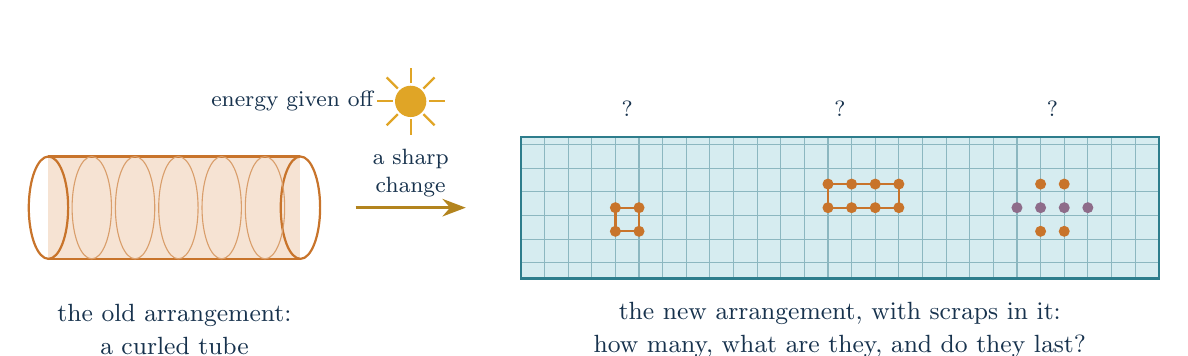
\begin{tikzpicture}[x=1cm,y=1cm,>=Stealth,font=\small]
% --- the old arrangement: the tube
\begin{scope}[shift={(0,0)}]
\fill[curlpale] (0,0.35) rectangle (3.2,1.65);
\draw[curl,thick] (0,0.35) -- (3.2,0.35) (0,1.65) -- (3.2,1.65);
\draw[curl,thick] (0,1) ellipse (0.25 and 0.65);
\draw[curl,thick] (3.2,1) ellipse (0.25 and 0.65);
\foreach \x in {0.55,1.1,...,2.8} {\draw[curl!70] (\x,1) ellipse (0.25 and 0.65);}
\node[text=ink,align=center] at (1.6,-0.55) {the old arrangement:\\a curled tube};
\end{scope}
% --- the change
\draw[->,very thick,sun!80!black] (3.9,1) -- (5.3,1) node[midway,above,text=ink,align=center,font=\footnotesize] {a sharp\\change};
\node[circle,fill=sun,inner sep=4pt] (sun) at (4.6,2.35) {};
\foreach \a in {0,45,...,315} {\draw[sun,thick] (sun) ++(\a:0.23) -- ++(\a:0.2);}
\node[text=ink,font=\footnotesize,anchor=east] at (4.25,2.35) {energy given off};
% --- the new arrangement, with leftovers
\begin{scope}[shift={(6.0,0)}]
\fill[flatpale] (0,0.1) rectangle (8.1,1.9);
\draw[flat!55,step=0.3] (0,0.1) grid (8.1,1.9);
\draw[flat,thick] (0,0.1) rectangle (8.1,1.9);
% leftover 1
\foreach \p in {(1.2,0.7),(1.5,0.7),(1.2,1.0),(1.5,1.0)} {\fill[curl] \p circle (0.07);}
\draw[curl,thick] (1.2,0.7) rectangle (1.5,1.0);
% leftover 2
\foreach \p in {(3.9,1.0),(4.2,1.0),(3.9,1.3),(4.2,1.3),(4.5,1.0),(4.5,1.3),(4.8,1.0),(4.8,1.3)} {\fill[curl] \p circle (0.07);}
\draw[curl,thick] (3.9,1.0) rectangle (4.8,1.3);
% leftover 3
\foreach \p in {(6.6,0.7),(6.9,0.7),(6.6,1.3),(6.9,1.3)} {\fill[curl] \p circle (0.07);}
\foreach \p in {(6.3,1.0),(6.6,1.0),(6.9,1.0),(7.2,1.0)} {\fill[melt] \p circle (0.07);}
\node[text=ink,font=\footnotesize] at (4.05,2.25) {?};
\node[text=ink,font=\footnotesize] at (1.35,2.25) {?};
\node[text=ink,font=\footnotesize] at (6.75,2.25) {?};
\node[text=ink,align=center] at (4.05,-0.55) {the new arrangement, with scraps in it:\\how many, what are they, and do they last?};
\end{scope}
\end{tikzpicture}
\caption{The question in one picture. \Sketch\ A curled arrangement changes sharply into a new one and
gives off energy. Small pieces are left over. This paper counts them, reads what they are, and follows
them while their surroundings stay warm or cool down.}
\label{fig:idea}
\end{figure}

\sub{Who is saying what}
The project keeps four kinds of statement apart, and this edition tags them where it matters.
\begin{itemize}\setlength{\itemsep}{1pt}
\item \Exact\ Arithmetic, or a reading of a saved network link by link. True of the toy whatever a
run does.
\item \Meas\ A simulation whose rules and predictions were written down before it ran, with its
verdict. \MeasX\ means a closer look at runs already read, with no prediction written first.
\item \Pub\ Other researchers' published results.
\item \Ours\ A reading of a result, offered by the author and her AI assistants and checked by no
physicist. \Claim\ The author's hypothesis about reality, stated as hers.
\end{itemize}
Numbers in square brackets point to the sources listed at the end.

\chapterpage{1 \enspace THE STORY SO FAR}{A tube of dots that burps}

This chapter repeats, briefly, what the first paper established~\cite{paper1}. A reader who has that
paper fresh can skip to Chapter~2.

\sub{The toy}
\Pub\ The toy is a network: dots joined by links, every dot holding exactly four links. It comes from
a published model in which space is not a stage but an arrangement of such a network
\cite{T17,KTB19,T25}. Four dots joined in a loop make a \textbf{square}. The toy gives every network
an energy by counting squares, and the whole rule is a price list of two lines: a missing square
costs 16 units, and a link that carries more than two squares pays extra for each surplus one.

The extra price is set by a number we call \textbf{the knob}. With the knob at 1 the toy is the
published model. Every result in this paper has the knob at 1.25, where a surplus square costs 5
units. That setting is our addition, so this toy is a close cousin of the published model and not the
model itself.

The toy changes by one kind of move, a \textbf{swap}: two links trade partners. A run is a long chain
of swaps, each proposed at random and then accepted or refused.

\sub{The tube, and its burp}
\Exact\ Wrap a square grid of dots into a tube only four dots around and join its ends. Every ring of
four dots around the tube is itself a square, so every link around the tube carries a surplus square
and pays for it. Call this \textbf{the curled tube}. It costs exactly 1 unit per dot more than an
arrangement in which every link carries two squares, which costs nothing at all.

So a lower arrangement exists. But no single swap leads toward it: a swap either leaves the tube's
energy where it was or costs at least 12 units. The tube is stable for now. \MeasX\ Given 12 units,
every tube tested left, and with less none did. The change then spreads along the tube until every dot
has been through it, giving off 1 unit for each dot. That release, and the event that gives it off, is the burp.

\sub{What the tube turns into}
\Exact\ Here is the first paper's least expected result. Read link by link, 98 of every 100 runs that
finished with nothing left over had turned the curled tube into another tube. Its seam has slipped by
two dots, so that going around it now takes six steps where it took
four. Six around is the least a tube can be without paying for surplus squares, so the new tube costs
nothing. Around every dot the squares fit together as they do on a flat sheet of graph paper, and we
call an arrangement like that \textbf{flat}. Flat describes what a dot sees close by. It says nothing
about how wide the tube is.

The seam could slip further, by four dots or six, and the tube would be eight or ten around, also at no
cost. Runs that finished clean almost never did that; runs that kept a scrap sometimes did, in part of
the tube. Like the first paper, this one mostly follows the tube six around. Chapter~8 comes back to the
other widths.

\begin{center}
\renewcommand{\arraystretch}{1.15}
\begin{tabular}{lrr}
\toprule
A tube of 96 dots & what it costs & what it has given off\\
\midrule
curled, four around & 96 units & nothing yet\\
after the burp, six around, no scrap & 0 units & 96 units\\
after the burp, six around, one common scrap & 14 units & 82 units\\
\bottomrule
\end{tabular}
\end{center}

The last line of that table is this paper's subject. \Meas\ In the first paper's runs the change
usually stopped one small piece short of finishing, leaving a scrap.

\takeaway{A curled tube of dots is stable for now. Given a small push it changes all at once into a
wider tube, six around, and gives off 1 unit of energy per dot: the burp. The change usually leaves
a scrap.}

\chapterpage{2 \enspace THE SCRAP}{What a single change leaves behind}

\sub{Read the wiring, not the count}
A run reports numbers: how many squares, how many dots that look flat. It is tempting to name a shape
from those numbers. This project has done that five times and been wrong five times. So every
statement below about what a scrap \emph{is} comes from reading a saved network link by link.

\Exact\ The common scrap is a closed loop of four dots that still closes a square, as each ring of
the old tube did. It is still curled, in that sense, but it does not go around the new tube: it lies
in the tube's wall. Six of the links at its dots carry a third square. At our knob setting it holds 14
units, which is the burp of fourteen dots, held back. We call it a \textbf{curled loop}.

\begin{figure}[H]
\centering
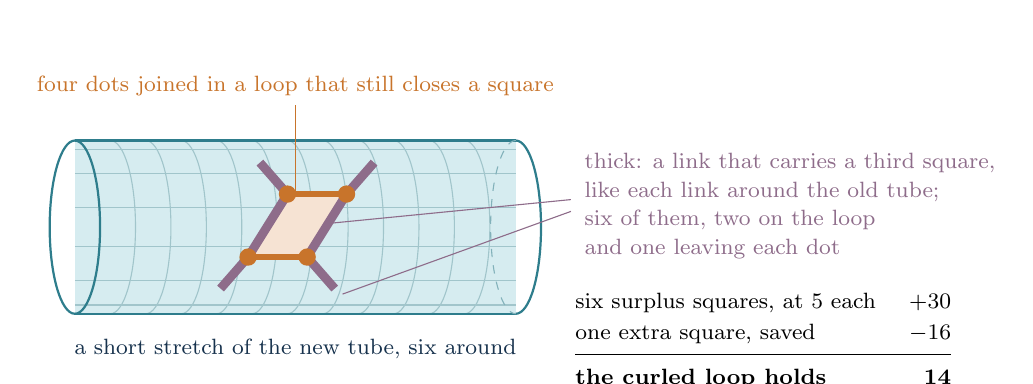
\begin{tikzpicture}[x=1cm,y=1cm,font=\footnotesize,>=Stealth]
% the new tube, a short stretch of it, drawn as a pipe
\fill[flatpale] (0,-1.1) rectangle (5.6,1.1);
\foreach \t in {-64,-38,-13,13,38,64} {\draw[flat!45] (0,{1.1*sin(\t)}) -- (5.6,{1.1*sin(\t)});}
\foreach \x in {0.45,0.9,...,5.2} {\draw[flat!45] (\x,1.1) arc (90:-90:0.32 and 1.1);}
\draw[flat,thick] (0,-1.1) -- (5.6,-1.1) (0,1.1) -- (5.6,1.1);
\draw[flat,thick] (0,0) ellipse (0.32 and 1.1);
\draw[flat,thick] (5.6,1.1) arc (90:-90:0.32 and 1.1);
\draw[flat!60,dashed] (5.6,1.1) arc (90:270:0.32 and 1.1);
% the scrap on its wall: a closed loop of four dots
\fill[curlpale] (2.2,-0.38) -- (2.95,-0.38) -- (3.45,0.42) -- (2.7,0.42) -- cycle;
\draw[curl,line width=2pt] (2.2,-0.38) -- (2.95,-0.38);
\draw[curl,line width=2pt] (2.7,0.42) -- (3.45,0.42);
\draw[melt,line width=3.2pt] (2.95,-0.38) -- (3.45,0.42);
\draw[melt,line width=3.2pt] (2.2,-0.38) -- (2.7,0.42);
\foreach \p/\q in {{(2.2,-0.38)}/{(1.85,-0.78)},{(2.95,-0.38)}/{(3.3,-0.78)},{(3.45,0.42)}/{(3.8,0.82)},{(2.7,0.42)}/{(2.35,0.82)}} {\draw[melt,line width=3.2pt] \p -- \q;}
\foreach \p in {(2.2,-0.38),(2.95,-0.38),(3.45,0.42),(2.7,0.42)} {\fill[curl] \p circle (0.11);}
% callouts
\draw[curl] (2.8,0.42) -- (2.8,1.55);
\node[text=curl,anchor=south,align=center] at (2.8,1.55) {four dots joined in a loop that still closes a square};
\draw[melt] (3.25,0.05) -- (6.3,0.35);
\draw[melt] (3.4,-0.85) -- (6.3,0.2);
\node[text=melt,anchor=west,align=left] at (6.35,0.27) {thick: a link that carries a third square,\\like each link around the old tube;\\six of them, two on the loop\\and one leaving each dot};
\node[text=ink,align=center] at (2.8,-1.55) {a short stretch of the new tube, six around};
% the bill
\node[anchor=north west,inner sep=0pt] at (6.35,-0.75) {\renewcommand{\arraystretch}{1.1}\begin{tabular}{@{}lr@{}}
six surplus squares, at 5 each & $+30$\\
one extra square, saved & $-16$\\ \midrule
\textbf{the curled loop holds} & \textbf{14}\\ \end{tabular}};
\end{tikzpicture}
\caption{The common scrap, link by link. \Exact\ The wiring and the bill. Read from the saved
networks of the first paper's maps and this paper's large test, 1,094 of 2,045 four-dot scraps are
wired this way. Most of the rest are a lighter kind, 4 units, in which all four sides of the loop carry
a third square and no link leaving it does; a few have five surplus squares and hold 9. None of the
2,045 goes around the new tube. \Sketch\ Where the loop sits on the tube is drawn to show its size. The
network has no positions, and the tube is too narrow for a picture of the fabric around the scrap to
be read off the wiring.}
\label{fig:loop}
\end{figure}

\sub{One push, about one scrap}
To follow the energy to the last unit, the first paper sealed the toy in a box. \Exact\ A
\textbf{sealed} run has no outside. Beside the network sit \textbf{stores}, each holding some units.
A swap that costs energy is paid from a store, and a swap that gives energy off pays into one.
Network plus stores never changes, and that was checked in every run. With two stores for every dot,
the burp spreads so thin that the box stays cold.

\Meas\ Eighty tubes were sealed in cold boxes, twenty each at 64, 96, 192 and 288 dots, and each was
given one 12-unit push, so that the change began in one place. We call a place where the change begins
a \textbf{start}. The prediction written down beforehand was that a longer tube leaves more
scraps. It does not. The count was 0.90, 0.85, 1.05 and 0.95 scraps per tube.

\begin{figure}[H]
\centering
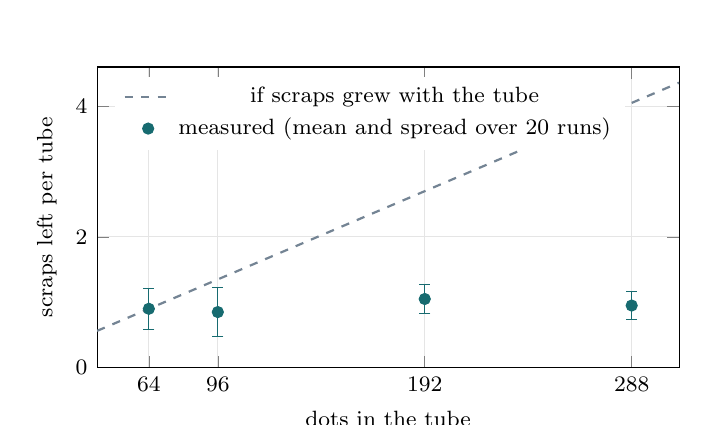
\begin{tikzpicture}
\begin{axis}[width=0.74\linewidth,height=5.4cm,xlabel={dots in the tube},ylabel={scraps left per tube},xmin=40,xmax=310,ymin=0,ymax=4.6,xtick={64,96,192,288},grid=both,grid style={gray!20},tick label style={font=\footnotesize},label style={font=\footnotesize},legend style={at={(0.03,0.97)},anchor=north west,font=\footnotesize,draw=none}]
\addplot[ink!60,dashed,thick,domain=40:310] {0.9*x/64};
\addplot[accent,only marks,mark=*,mark options={fill=accent},error bars/.cd,y dir=both,y explicit] coordinates {(64,0.90) +- (0,0.31) (96,0.85) +- (0,0.37) (192,1.05) +- (0,0.22) (288,0.95) +- (0,0.22)};
\legend{if scraps grew with the tube, measured (mean and spread over 20 runs)}
\end{axis}
\end{tikzpicture}
\caption{One start, about one scrap. \Meas\ The dashed line is what a leftover growing in step with
the tube would look like. The measured counts sit flat. The prediction that they would grow failed.}
\label{fig:one}
\end{figure}

\Meas\ A second test asked where the scrap sits. Two guesses were written down: at the place the
change started, or at the far side, where the change spreading both ways around the tube would meet
itself. It sits at neither. Its position is spread evenly along the tube. So this scrap is not a seam
where the change met itself. We call a scrap that sits inside the new tube, away from any meeting
place, a \textbf{free scrap}.

\MeasX\ In 9 of the 80 boxes the leftover was not a curled loop. It was a different object holding 20
units, which the first paper called a twist. It comes back in Chapter~7.

\takeaway{A change that starts in one place leaves about one scrap, whatever the size of the tube,
and the scrap can sit anywhere: it is a free scrap. The common one is a curled loop of four dots
holding 14 units, and it is not the only kind.}

\chapterpage{3 \enspace MORE STARTS}{Does every start leave a scrap?}

A change in a large space need not start in one place. So the next question is what several starts
leave.

\sub{Starts planted by hand}
From each start the change spreads both ways
along the tube. The moving edge between changed and unchanged tube is a \textbf{front}, and where two
fronts meet, two changed stretches join.

\Meas\ A tube of 384 dots was sealed in a cold box, and the change was started by hand at one, two,
four or eight evenly spaced places, twenty runs each. The author's hypothesis fits one scrap per
start. Another guess, which the last chapter invites, is one scrap per tube, however many starts.
Neither held.

\begin{figure}[H]
\centering
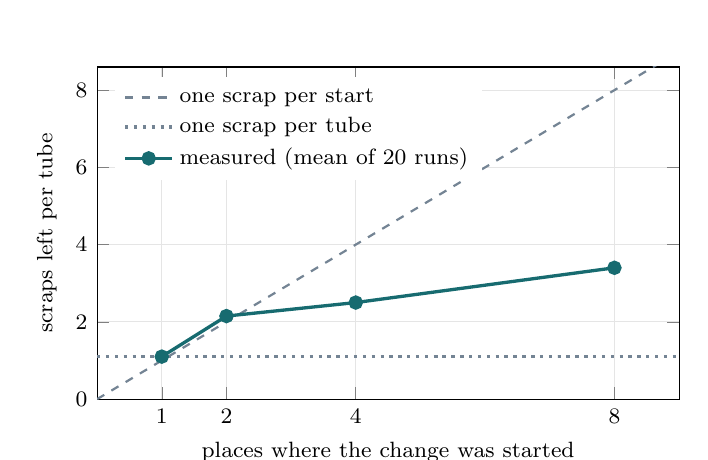
\begin{tikzpicture}
\begin{axis}[width=0.74\linewidth,height=5.8cm,xlabel={places where the change was started},ylabel={scraps left per tube},xmin=0,xmax=9,ymin=0,ymax=8.6,xtick={1,2,4,8},ytick={0,2,4,6,8},grid=both,grid style={gray!20},tick label style={font=\footnotesize},label style={font=\footnotesize},legend style={at={(0.03,0.97)},anchor=north west,font=\footnotesize,draw=none},legend cell align=left]
\addplot[ink!60,dashed,thick,domain=0:9] {x};
\addplot[ink!60,dotted,very thick,domain=0:9] {1.1};
\addplot[accent,very thick,mark=*,mark options={fill=accent}] coordinates {(1,1.10) (2,2.15) (4,2.50) (8,3.40)};
\legend{one scrap per start, one scrap per tube, measured (mean of 20 runs)}
\end{axis}
\end{tikzpicture}
\caption{More starts, more scraps, but fewer than one each. \Meas\ One start left 1.10 scraps on
average, two left 2.15, four left 2.50 and eight left 3.40. Both guesses written down beforehand,
one per start and one per tube, failed.}
\label{fig:starts}
\end{figure}

\sub{Tubes that start themselves}
Nobody plants starts in a large space. To see what a tube does on its own, we need the other way of
running the toy.

\Pub\ Instead of a sealed box, picture the network sitting in a \textbf{bath} that lends it energy
for a swap that costs and takes back what a swap gives off. The bath is endless. One number sets how
freely it lends, and we call that number \textbf{the warmth}. In a warm bath costly swaps happen
often. In a cold one they almost never do. Time in a run is counted in \textbf{sweeps}: one sweep is
two proposed swaps for every dot.

In a bath the curled tube needs no push. Sooner or later the bath lends the 12 units somewhere, and
the change starts there. In a long tube it starts in several places before any one change has
crossed the tube.

\Meas\ Tubes of 256 to 4,096 dots were left in baths at three warmths. Three predictions written down
beforehand held: longer tubes start in more places, the changed share grows over time the way the
textbook law for changes that start at random places and spread says it should~\cite{KJMA}, and
longer tubes are left holding more energy.

\Meas\ A later, larger test let tubes of 512, 1,024 and 2,048 dots start themselves at the coldest of
those warmths and counted the curled loops left when the change was over.

\begin{figure}[H]
\centering
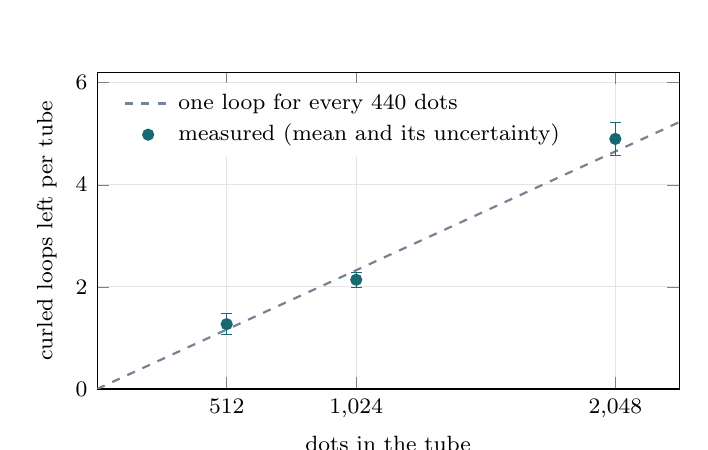
\begin{tikzpicture}
\begin{axis}[width=0.74\linewidth,height=5.6cm,xlabel={dots in the tube},ylabel={curled loops left per tube},xmin=0,xmax=2300,ymin=0,ymax=6.2,xtick={512,1024,2048},xticklabels={512,{1,024},{2,048}},grid=both,grid style={gray!20},tick label style={font=\footnotesize},label style={font=\footnotesize},legend style={at={(0.03,0.97)},anchor=north west,font=\footnotesize,draw=none},legend cell align=left,scaled x ticks=false]
\addplot[ink!60,dashed,thick,domain=0:2300] {x/440};
\addplot[accent,only marks,mark=*,mark options={fill=accent},error bars/.cd,y dir=both,y explicit] coordinates {(512,1.27) +- (0,0.21) (1024,2.14) +- (0,0.15) (2048,4.90) +- (0,0.33)};
\legend{one loop for every 440 dots, measured (mean and its uncertainty)}
\end{axis}
\end{tikzpicture}
\caption{A tube that starts itself leaves scraps in step with its length. \Meas\ 1.27, 2.14 and 4.90
curled loops per tube at 512, 1,024 and 2,048 dots: about one for every 400 to 480 dots. From 40, 80
and 40 tubes.}
\label{fig:length}
\end{figure}

So the single scrap of Chapter~2 is what a single start leaves. A tube long enough to start in many
places leaves scraps in proportion to its length.

\sub{A warning about warm baths}
\Meas\ The longest tubes in the two warmest baths did something else. More than half of their dots
ended with too few squares around them, and the tubes had taken in about twice as much energy from
the bath as a burp gives off. That is \textbf{melting}: the bath breaks squares faster than the toy
re-forms them, and the network ends up linked any old way. \Exact\ A sealed tube cannot melt. Its own
burp holds enough energy to break at most one square in sixteen. Melting needs energy from outside.

\takeaway{More starts leave more scraps, but fewer than one each. A tube long enough to start itself
in many places leaves about one curled loop for every 400 to 480 dots.}

\chapterpage{4 \enspace WARMTH}{Does a scrap last if its surroundings stay warm?}

\Meas\ New tubes of 96 dots were changed in cold sealed boxes, and those left holding exactly one
curled loop were moved into a bath and held at one warmth for 100,000 sweeps. Three warmths were
tried. Three outcomes were written down beforehand: the scrap wanders, or it heals in the warmer
baths and stays in the colder, or it stays everywhere. To \textbf{heal} means that the scrap's dots
rearrange into the flat pattern around them and its energy is given off.

It healed at every warmth.

\begin{figure}[H]
\centering
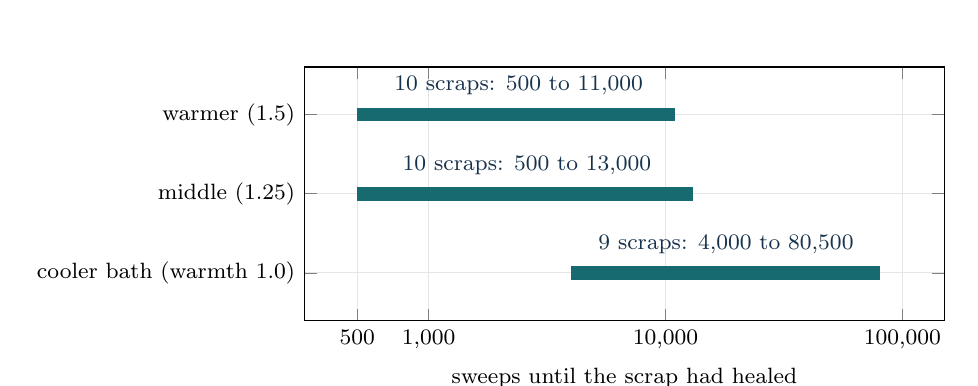
\begin{tikzpicture}
\begin{axis}[width=0.8\linewidth,height=4.8cm,xmode=log,xlabel={sweeps until the scrap had healed},xmin=300,xmax=150000,ymin=0.4,ymax=3.6,ytick={1,2,3},yticklabels={{cooler bath (warmth 1.0)},{middle (1.25)},{warmer (1.5)}},xtick={500,1000,10000,100000},xticklabels={500,{1,000},{10,000},{100,000}},grid=both,grid style={gray!20},tick label style={font=\footnotesize},label style={font=\footnotesize}]
\addplot[accent,line width=5pt] coordinates {(4000,1) (80500,1)};
\addplot[accent,line width=5pt] coordinates {(500,2) (13000,2)};
\addplot[accent,line width=5pt] coordinates {(500,3) (11000,3)};
\node[font=\footnotesize,text=ink,anchor=south] at (axis cs:18000,1.12) {9 scraps: 4,000 to 80,500};
\node[font=\footnotesize,text=ink,anchor=south] at (axis cs:2600,2.12) {10 scraps: 500 to 13,000};
\node[font=\footnotesize,text=ink,anchor=south] at (axis cs:2400,3.12) {10 scraps: 500 to 11,000};
\end{axis}
\end{tikzpicture}
\caption{How long a lone curled loop lasted in a bath. \Meas\ Each bar runs from the first scrap healed
to the last. The scrap's position was read every 500 sweeps, so 500 is the shortest time the test
could report. Even the coolest bath healed every one, in time.}
\label{fig:heal}
\end{figure}

\Meas\ Two things about how it healed. Each tube held one scrap, so each scrap healed by itself, with
nothing to meet. And 27 of the 29 were never seen to move first. A curled loop mostly sits where it
is until it is gone.

In the cold sealed boxes of Chapter~2, by contrast, every scrap lasted the whole run.

\takeaway{A lone curled loop heals away in every bath we tried, in 500 to 80,500 sweeps. It lasts
only where its surroundings are very cold.}

\chapterpage{5 \enspace THE RACE}{What if the surroundings cool down?}

Warm surroundings heal a scrap and cold ones keep it. Reality cooled as it expanded. So what matters
for a remainder is a race: does the scrap heal before its surroundings get too cold to heal it?

\Meas\ Tubes of 96 dots, each holding one curled loop, were put in a bath at warmth 1.25, where the
last chapter saw every scrap heal within 13,000 sweeps. The bath was then cooled, in equal steps, to
a warmth of 0.25, where no swap is ever accepted, and held there. The cooling was spread over anything
from 300 to 100,000 sweeps. The verdict written down beforehand was \emph{freezes in} if some cooling
time keeps most scraps and the fastest cooling keeps the most.

\begin{figure}[H]
\centering
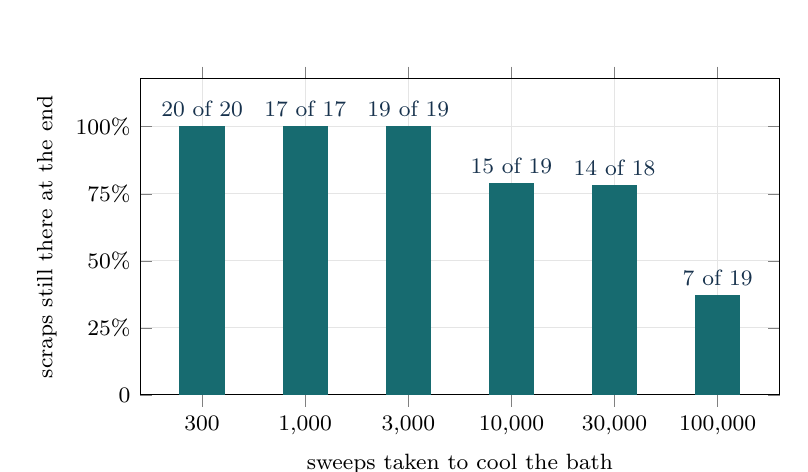
\begin{tikzpicture}
\begin{axis}[width=0.8\linewidth,height=5.6cm,ybar,bar width=16pt,xlabel={sweeps taken to cool the bath},ylabel={scraps still there at the end},xmin=0.4,xmax=6.6,ymin=0,ymax=118,xtick={1,2,3,4,5,6},xticklabels={300,{1,000},{3,000},{10,000},{30,000},{100,000}},ytick={0,25,50,75,100},yticklabels={0,25\%,50\%,75\%,100\%},grid=both,grid style={gray!20},tick label style={font=\footnotesize},label style={font=\footnotesize},nodes near coords,nodes near coords style={font=\footnotesize,text=ink},point meta=explicit symbolic]
\addplot[fill=accent,draw=accent] coordinates {(1,100) [20 of 20] (2,100) [17 of 17] (3,100) [19 of 19] (4,79) [15 of 19] (5,78) [14 of 18] (6,37) [7 of 19]};
\end{axis}
\end{tikzpicture}
\caption{Cooling keeps a scrap that warmth would have healed. \Meas\ Every scrap survived a fast
cooling. About four in five survived a cooling of 10,000 or 30,000 sweeps. A third survived the
slowest.}
\label{fig:race}
\end{figure}

It freezes in. Even a cooling of 30,000 sweeps, more than twice the longest healing time at the
starting warmth, kept most scraps, because the bath leaves the range where healing is quick early in
the cooling. The scraps that healed did so in the first 15,000 sweeps.

\takeaway{A scrap that would heal in any warm bath survives if the bath cools, even slowly. Cooling
freezes it in.}

\chapterpage{6 \enspace THE LARGE TEST}{Many scraps, cooled slowly}

The last three chapters used small tubes and one scrap at a time. This chapter puts the pieces
together: tubes large enough to start themselves in many places, left with several scraps each, and
then cooled.

\sub{A fair clock}
One thing has to be fixed first. A swap needs two particular links to be picked together. In a
network ten times larger, any particular pair is picked a tenth as often in a sweep. So anything
local, like a scrap healing, takes more sweeps in a bigger network for no reason but bookkeeping. To
compare sizes we count time in \textbf{fair sweeps}, the fair clock of the first paper's Chapter~5:
sweeps scaled so that each small neighborhood gets as many chances as it would in a 96-dot network. At
1,024 dots one fair sweep is about eleven sweeps. The clock decides how a cooling time at one size
compares with a cooling time at another. No energy, and no reading of a scrap's wiring, depends on it.

\sub{The test}
\Meas\ Eighty tubes of 1,024 dots were left in a bath at warmth 1.25 until the change was over. Each
finished tube was then copied, and the copies were cooled at seven speeds, from an instant chill to a
cooling spread over 300,000 fair sweeps. So every cooling speed began from the very same tubes. The
slowest cooling used the first forty.

The question written down beforehand was the \emph{shape} of the fall. Does each tenfold slowing of
the cooling lose a steady fraction of the curled loops (a gentle fall), or does the count hold and
then collapse (a cliff)? The author predicted a gentle fall.

\begin{figure}[H]
\centering
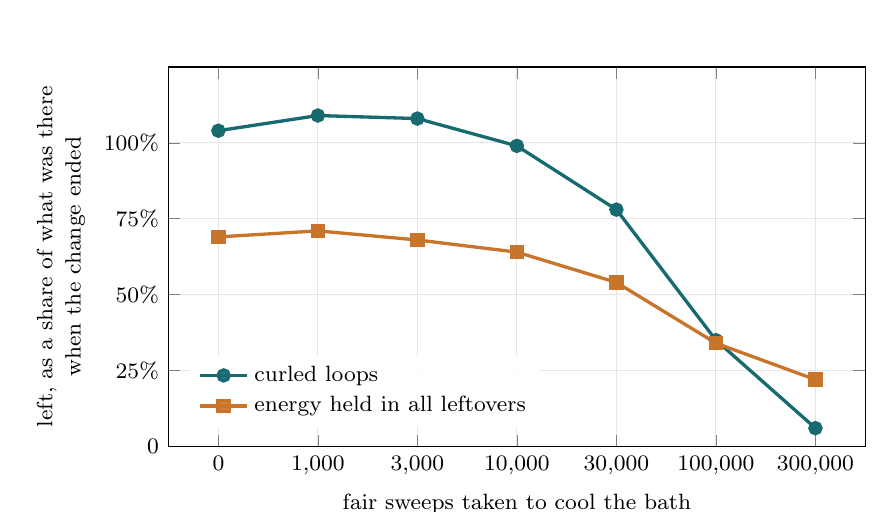
\begin{tikzpicture}
\begin{axis}[width=0.86\linewidth,height=6.4cm,xlabel={fair sweeps taken to cool the bath},ylabel={left, as a share of what was there\\when the change ended},ylabel style={align=center},xmin=0.5,xmax=7.5,ymin=0,ymax=125,xtick={1,2,3,4,5,6,7},xticklabels={0,{1,000},{3,000},{10,000},{30,000},{100,000},{300,000}},ytick={0,25,50,75,100},yticklabels={0,25\%,50\%,75\%,100\%},grid=both,grid style={gray!20},tick label style={font=\footnotesize},label style={font=\footnotesize},legend style={at={(0.03,0.05)},anchor=south west,font=\footnotesize,draw=none,fill=white,fill opacity=0.9,text opacity=1},legend cell align=left]
\addplot[accent,very thick,mark=*,mark options={fill=accent}] coordinates {(1,104) (2,109) (3,108) (4,99) (5,78) (6,35) (7,6)};
\addplot[curl,very thick,mark=square*,mark options={fill=curl}] coordinates {(1,69) (2,71) (3,68) (4,64) (5,54) (6,34) (7,22)};
\legend{curled loops, energy held in all leftovers}
\end{axis}
\end{tikzpicture}
\caption{The curled loops fall off a cliff. The energy does not follow them. \Meas\ Slowing the
cooling from 10,000 to 100,000 fair sweeps lost two curled loops in three. Slowing it from 30,000 to
300,000 lost twelve in thirteen. The energy held in leftovers fell far less. About three units in ten of
that energy go in any cooling, even an instant chill, as loose small pieces settle. The loop count can
start above 100\% because a few loops form after the first count.}
\label{fig:cliff}
\end{figure}

A cliff. The prediction failed.

\sub{The energy that stays is not in the curled loops}
\Meas\ If curled loops were the only leftovers, the energy held in leftovers would have fallen with
them. It did not. After the slowest cooling, 6 curled loops in 100 were left, and 22 units in 100 of
the leftover energy. Something else was holding energy, and cooling slowly did nothing to it.

\begin{figure}[H]
\centering
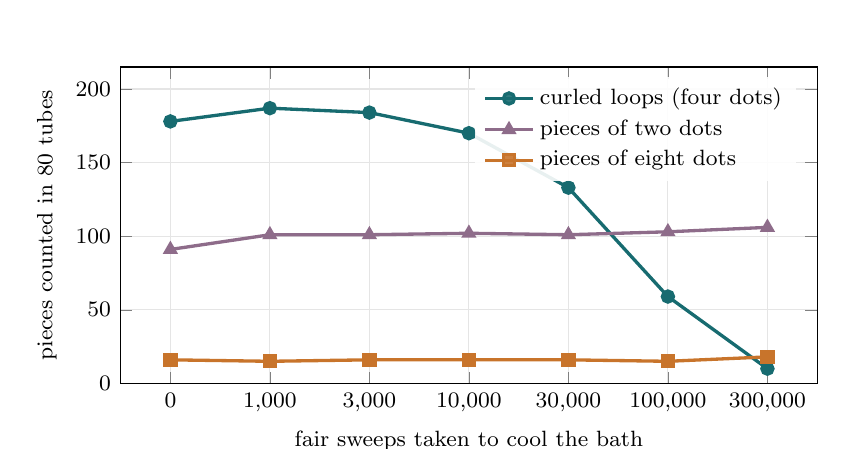
\begin{tikzpicture}
\begin{axis}[width=0.86\linewidth,height=5.6cm,xlabel={fair sweeps taken to cool the bath},ylabel={pieces counted in 80 tubes},xmin=0.5,xmax=7.5,ymin=0,ymax=215,xtick={1,2,3,4,5,6,7},xticklabels={0,{1,000},{3,000},{10,000},{30,000},{100,000},{300,000}},grid=both,grid style={gray!20},tick label style={font=\footnotesize},label style={font=\footnotesize},legend style={at={(0.97,0.97)},anchor=north east,font=\footnotesize,draw=none,fill=white,fill opacity=0.9,text opacity=1},legend cell align=left]
\addplot[accent,very thick,mark=*,mark options={fill=accent}] coordinates {(1,178) (2,187) (3,184) (4,170) (5,133) (6,59) (7,10)};
\addplot[melt,very thick,mark=triangle*,mark options={fill=melt}] coordinates {(1,91) (2,101) (3,101) (4,102) (5,101) (6,103) (7,106)};
\addplot[curl,very thick,mark=square*,mark options={fill=curl}] coordinates {(1,16) (2,15) (3,16) (4,16) (5,16) (6,15) (7,18)};
\legend{curled loops (four dots), pieces of two dots, pieces of eight dots}
\end{axis}
\end{tikzpicture}
\caption{What slow cooling removes, and what it does not. \Meas\ Leftover pieces sorted by how many
dots they hold. The curled loops fall away. The pieces of two and of eight do not change at all
across the whole range. The slowest cooling was run on forty tubes and
its counts are doubled here.}
\label{fig:kinds}
\end{figure}

\sub{Two checks on the test itself}
\Meas\ The fair clock made a prediction of its own: counted in fair sweeps, the 1,024-dot tubes
should lose their curled loops at the same pace the 96-dot tubes of Chapter~5 did. At one of the two
points checked they lost them sooner, by more than the margin allowed. So the fair clock is a better
ruler than plain sweeps and still not an exact one. The second check held: at one cooling speed,
tubes of 512, 1,024 and 2,048 dots kept the same number of curled loops for their length.

\whyhere{Chapters 4 and 5 said a scrap heals in warmth and freezes in when cooled. That left the
question that matters for a remainder: across many scraps, how much is frozen in, and how does that
depend on the speed of cooling? The answer was not the one predicted, and it pointed at leftovers
nobody had looked at.}

\takeaway{Cooled slowly enough, nearly all the curled loops heal. Most of the leftover energy stays
anyway, held by smaller and larger pieces that no cooling we ran removed.}

\chapterpage{7 \enspace A CLOSER LOOK}{What are the pieces that stay?}

\sub{Three guesses, written down first}
Before anyone read the pieces of two and of eight, three guesses about them were written down, with a
test for each.

\begin{itemize}\setlength{\itemsep}{1pt}
\item \textbf{A scar}: damage that one swap would mend, if the bath ever offered that swap. The test:
is there a single swap that removes the piece and lowers the energy?
\item \textbf{A seam}: the stitching where two stretches of new tube, grown from different starts,
met and did not match. The test: does the piece hold a link joining two places that are otherwise far
apart?
\item \textbf{Stuck on its own}: a small arrangement that sits in a dip of its own, so that every
swap out of it costs energy. The registered name for this guess was KNOT.
\end{itemize}

The author predicted a seam.

\Exact\ All 600 saved tubes were read link by link. Not one piece of any size can be mended by a
single swap. Of 2,121 pieces, 4 hold a far-reaching link. \Meas\ The verdict was the third guess:
stuck on its own. The author's prediction failed.

\sub{Three kinds of scrap}
\Exact\ Read from the wiring, the leftovers are three objects.

\begin{figure}[H]
\centering
% a short stretch of the new tube drawn as a pipe, at x-offset #1
\newcommand{\pipe}[1]{%
\begin{scope}[shift={(#1,0)}]
\fill[flatpale] (0,-1.0) rectangle (4.0,1.0);
\foreach \t in {-62,-36,-12,12,36,62} {\draw[flat!45] (0,{1.0*sin(\t)}) -- (4.0,{1.0*sin(\t)});}
\foreach \x in {0.4,0.8,...,3.7} {\draw[flat!45] (\x,1.0) arc (90:-90:0.28 and 1.0);}
\draw[flat,thick] (0,-1.0) -- (4.0,-1.0) (0,1.0) -- (4.0,1.0);
\draw[flat,thick] (0,0) ellipse (0.28 and 1.0);
\draw[flat,thick] (4.0,1.0) arc (90:-90:0.28 and 1.0);
\draw[flat!60,dashed] (4.0,1.0) arc (90:270:0.28 and 1.0);
\end{scope}}
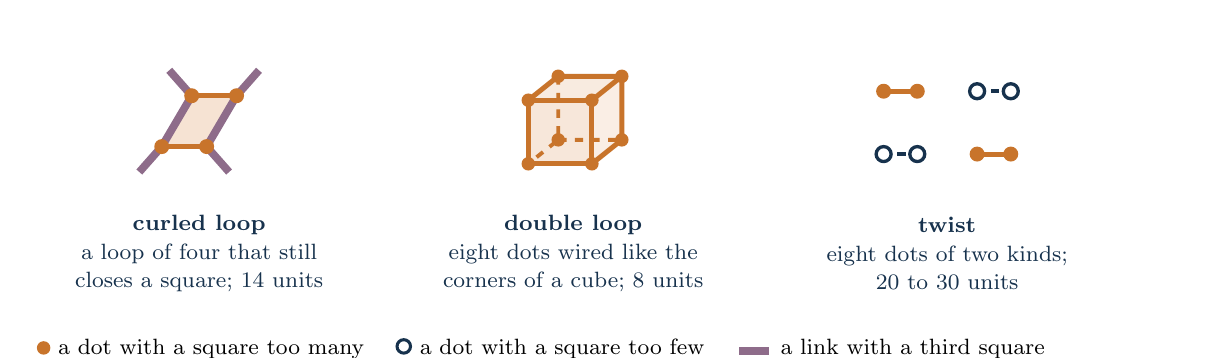
\begin{tikzpicture}[x=0.95cm,y=0.95cm,font=\footnotesize]
% ---------- the curled loop
\pipe{0}
\fill[curlpale] (1.5,-0.32) -- (2.1,-0.32) -- (2.5,0.36) -- (1.9,0.36) -- cycle;
\draw[curl,line width=1.8pt] (1.5,-0.32) -- (2.1,-0.32) (1.9,0.36) -- (2.5,0.36);
\draw[melt,line width=2.8pt] (2.1,-0.32) -- (2.5,0.36) (1.5,-0.32) -- (1.9,0.36);
\foreach \p/\q in {{(1.5,-0.32)}/{(1.2,-0.66)},{(2.1,-0.32)}/{(2.4,-0.66)},{(2.5,0.36)}/{(2.8,0.7)},{(1.9,0.36)}/{(1.6,0.7)}} {\draw[melt,line width=2.8pt] \p -- \q;}
\foreach \p in {(1.5,-0.32),(2.1,-0.32),(2.5,0.36),(1.9,0.36)} {\fill[curl] \p circle (0.1);}
\node[text=ink,align=center] at (2.0,-1.75) {\textbf{curled loop}\\a loop of four that still\\closes a square; 14 units};
% ---------- the double loop: wired like the corners and edges of a cube
\pipe{5.0}
\begin{scope}[shift={(5.0,0)}]
\fill[curlpale,opacity=0.85] (1.4,-0.55) -- (2.25,-0.55) -- (2.25,0.3) -- (1.4,0.3) -- cycle;
\fill[curlpale!70,opacity=0.85] (2.25,-0.55) -- (2.65,-0.23) -- (2.65,0.62) -- (2.25,0.3) -- cycle;
\fill[curlpale!85,opacity=0.85] (1.4,0.3) -- (2.25,0.3) -- (2.65,0.62) -- (1.8,0.62) -- cycle;
\draw[curl,line width=1.4pt,dashed] (1.8,0.62) -- (1.8,-0.23) -- (1.4,-0.55) (1.8,-0.23) -- (2.65,-0.23);
\draw[curl,line width=1.8pt] (1.4,-0.55) -- (2.25,-0.55) -- (2.25,0.3) -- (1.4,0.3) -- cycle;
\draw[curl,line width=1.8pt] (2.25,-0.55) -- (2.65,-0.23) -- (2.65,0.62) -- (2.25,0.3) (2.65,0.62) -- (1.8,0.62) -- (1.4,0.3);
\foreach \p in {(1.4,-0.55),(2.25,-0.55),(2.25,0.3),(1.4,0.3),(1.8,-0.23),(2.65,-0.23),(2.65,0.62),(1.8,0.62)} {\fill[curl] \p circle (0.09);}
\node[text=ink,align=center] at (2.0,-1.75) {\textbf{double loop}\\eight dots wired like the\\corners of a cube; 8 units};
\end{scope}
% ---------- the twist: two pairs with a square too many, two with a square too few
\pipe{10.0}
\begin{scope}[shift={(10.0,0)}]
\draw[curl,line width=1.8pt] (1.15,0.42) -- (1.6,0.42) (2.4,-0.42) -- (2.85,-0.42);
\foreach \p in {(1.15,0.42),(1.6,0.42),(2.4,-0.42),(2.85,-0.42)} {\fill[curl] \p circle (0.1);}
\draw[ink,line width=1.4pt,densely dashed] (1.15,-0.42) -- (1.6,-0.42) (2.4,0.42) -- (2.85,0.42);
\foreach \p in {(1.15,-0.42),(1.6,-0.42),(2.4,0.42),(2.85,0.42)} {\filldraw[fill=white,draw=ink,line width=1.2pt] \p circle (0.1);}
\node[text=ink,align=center] at (2.0,-1.75) {\textbf{twist}\\eight dots of two kinds;\\20 to 30 units};
\end{scope}
% legend
\node[anchor=north west,align=left,text width=14.6cm] at (-0.3,-2.75) {%
\tikz\fill[curl] (0,0) circle (0.09); a dot with a square too many \quad
\tikz\filldraw[fill=white,draw=ink,line width=1.1pt] (0,0) circle (0.09); a dot with a square too few \quad
\tikz\draw[melt,line width=2.6pt] (0,0) -- (0.4,0); a link with a third square};
\end{tikzpicture}
\caption{The three kinds of scrap. \Exact\ How many dots, how they are wired, and what they hold, read
from the saved networks. The curled loop is the one of Figure~\ref{fig:loop}. The double loop's eight
dots have twelve links among them, three each, wired like the corners and edges of a cube: two loops of
four joined corner to corner, as two neighboring rings of the old tube were. In the twist, each orange dot
has two links that carry a third square, and each hollow dot has two links that carry only one. \Sketch\ Where each sits on the tube, and the pairs' arrangement, are drawn to
show the sizes.}
\label{fig:three}
\end{figure}

\begin{center}
\renewcommand{\arraystretch}{1.15}
\begin{tabular}{@{}lccc@{}}
\toprule
 & curled loop & double loop & twist\\
\midrule
dots & 4 & 8 & 8, of two kinds\\
holds & 14 units & 8 units & 20 to 30 units\\
cheapest swap out & costs 12 & costs 11 & costs 11\\
when cooled slowly & heals & stays & stays\\
\bottomrule
\end{tabular}
\end{center}

\textbf{What the three share.} \Exact\ Each is stuck on its own: every single swap out of it costs
energy. Each holds a fixed amount, set by its wiring and not by the size of the tube. Each was made by
the change, and almost none holds a link reaching far across the tube (4 pieces of 2,121). \textbf{What sets them apart} is their
size, what they hold, whether their dots have a square too many or also a square too few, and their
fate when cooled slowly. The count of leftover pieces in the last chapter split each twist into four
pieces of two dots, which is why so many pieces of two appeared. \Ours\ The 20-unit twist that turned
up in 9 of 80 boxes in Chapter~2 is the same kind of object. Whether it is wired exactly the same has
not been settled.

\sub{The same first step, a different fate}
\Exact\ The cheapest swap out of a curled loop costs 12 units. The cheapest swap out of a double loop
or a twist costs 11 in nearly every one read. Those are nearly the same. Yet the curled loop heals when
cooled slowly and the other two do not.

\Ours\ So the first step cannot be what decides. What decides must lie further along: after the first
costly swap, a curled loop must have a way downhill to the flat pattern, and the other two must not
have one within reach. Nobody has traced those paths. Until someone does, this paragraph is a guess.

\whyhere{A leftover named from a count has been wrong five times in this project. The pieces that
survived cooling were going to carry the paper's main result, so they were read from the wiring
before they were named, with the guesses and their tests written down first.}

\takeaway{The change leaves three kinds of scrap: the curled loop, the double loop and the twist. All
three are stuck on their own and hold a fixed amount, and none is a seam of the kind tested, a
far-reaching link. Leaving any of them costs about the same first step, yet only the curled loop
heals.}

\chapterpage{8 \enspace WHERE SCRAPS SIT}{Free scraps, and scraps that are joints}

Two tests so far said the scraps are not seams. The single scrap of Chapter~2 does not sit where the
change met itself, and almost no leftover in Chapter~7 holds a link reaching far across the tube. A
reading of the first paper's saved runs finds a seam of a different sort.

\sub{The new tube does not have to be six around}
\Exact\ Chapter~1 said the curled tube turns into a tube six around, its seam slipped by two dots.
The seam can slip further. Slip it by four and the tube is eight around. Slip it by six and it is ten
around. Every one of those costs nothing, because the toy charges for loops of four dots and for
nothing longer. So only the first slip, from four around to six, gives off energy, and nothing pushes
the change past it. Runs that finished clean almost always stopped there.

\MeasX\ The first paper saved the final network of 11,880 runs. In 2,014 of them the change had
finished with something left over. Those were read again, looking only at dots far enough from any
leftover to see clean flat pattern all around them, which shows how wide the tube is there.

\begin{center}
\renewcommand{\arraystretch}{1.15}
\begin{tabular}{@{}lr@{}}
\toprule
Of 2,014 finished runs with something left over & runs\\
\midrule
six around wherever it could be read & 774\\
wider than six wherever it could be read & 473\\
a stretch six around \emph{and} a wider stretch & 440\\
\quad of those, the two stretches touch directly & 0\\
the rest: too few clean dots, or counts that fit neither width & 327\\
\bottomrule
\end{tabular}
\end{center}

\Exact\ In all 440, a leftover lies between the stretch that is six around and the wider one.

\begin{figure}[H]
\centering
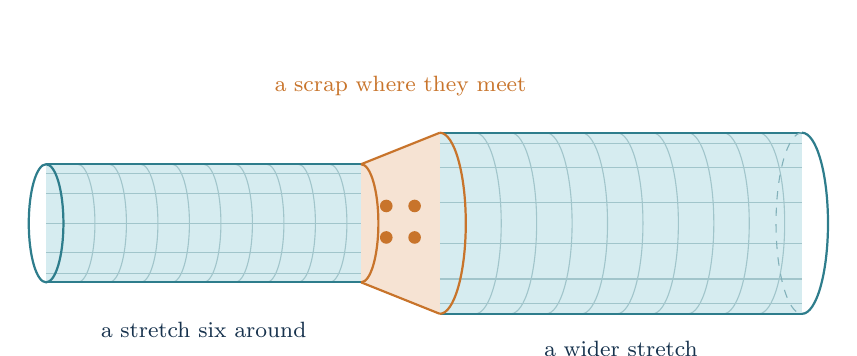
\begin{tikzpicture}[x=1cm,y=1cm,font=\small]
% the narrower stretch: six around
\fill[flatpale] (0,-0.75) rectangle (4.0,0.75);
\foreach \t in {-58,-30,0,30,58} {\draw[flat!45] (0,{0.75*sin(\t)}) -- (4.0,{0.75*sin(\t)});}
\foreach \x in {0.4,0.8,...,3.7} {\draw[flat!45] (\x,0.75) arc (90:-90:0.22 and 0.75);}
\draw[flat,thick] (0,-0.75) -- (4.0,-0.75) (0,0.75) -- (4.0,0.75);
\draw[flat,thick] (0,0) ellipse (0.22 and 0.75);
% the collar where they meet: the scrap
\fill[curlpale] (4.0,-0.75) -- (5.0,-1.15) -- (5.0,1.15) -- (4.0,0.75) -- cycle;
\draw[curl,thick] (4.0,-0.75) -- (5.0,-1.15) (4.0,0.75) -- (5.0,1.15);
\draw[curl,thick] (4.0,0.75) arc (90:-90:0.22 and 0.75);
\foreach \p in {(4.32,-0.18),(4.68,-0.18),(4.32,0.22),(4.68,0.22)} {\fill[curl] \p circle (0.08);}
% the wider stretch
\fill[flatpale] (5.0,-1.15) rectangle (9.6,1.15);
\foreach \t in {-62,-38,-13,13,38,62} {\draw[flat!45] (5.0,{1.15*sin(\t)}) -- (9.6,{1.15*sin(\t)});}
\foreach \x in {5.45,5.9,...,9.3} {\draw[flat!45] (\x,1.15) arc (90:-90:0.33 and 1.15);}
\draw[flat,thick] (5.0,-1.15) -- (9.6,-1.15) (5.0,1.15) -- (9.6,1.15);
\draw[curl,thick] (5.0,1.15) arc (90:-90:0.33 and 1.15);
\draw[flat,thick] (9.6,1.15) arc (90:-90:0.33 and 1.15);
\draw[flat!60,dashed] (9.6,1.15) arc (90:270:0.33 and 1.15);
\node[text=ink,font=\footnotesize,align=center] at (2.0,-1.35) {a stretch six around};
\node[text=ink,font=\footnotesize,align=center] at (7.3,-1.6) {a wider stretch};
\node[text=curl,font=\footnotesize,align=center] at (4.5,1.75) {a scrap where they meet};
\end{tikzpicture}
\caption{A scrap as a joint. \Sketch\ Narrower on the left, wider on the right; the widths are drawn to
suggest, not to scale. \Exact\ In every one of the 440 saved networks that hold both widths, the two
never meet directly. A leftover always sits between them.}
\label{fig:joint}
\end{figure}

\sub{Two places a scrap can sit}
So a scrap can sit in one of two places. A \textbf{free scrap} sits inside a stretch of one width, as
the scrap of Chapter~2 does. A \textbf{joint} sits where a stretch six around meets a wider one: a seam,
though not the kind Chapter~7 tested, since it needs no link reaching far across the tube. \MeasX\ Free
scraps are the common case. In about three of every five runs that kept a leftover, every leftover sat
inside one width; about one in five holds a joint. The first paper's sealed boxes with little room show
the same thing on a larger scale: patchworks of stretches six around and wider, with flaws frozen in
where the stretches meet~\cite{paper1}.

\Ours\ How a joint might come to be: two starts whose stretches slipped by different amounts, say by
two and by four, grow toward each other, and where they meet the wiring cannot match. A joint like that
may not be removable at all while the two stretches keep different widths, which would be a reason for
a scrap to last that has nothing to do with cooling. That is a reading of old runs, made after the
fact. Which of the three kinds of scrap are joints has not been read. Before it counts, it needs its own
prediction and fresh runs.

\takeaway{A scrap can be free, inside one width, or a joint, where a stretch six around meets a wider
one. Free scraps are the common case. Where a run holds two widths, a scrap always sits between them.}

\chapterpage{9 \enspace WHAT WE HAVE LEARNED, AND WHAT COMES NEXT}{The remainder that lasts is not the common one}

\sub{What is established in the toy}
A sharp change in this toy leaves small scraps of three kinds, each stuck on its own and each holding a
fixed amount. Most are free, sitting inside the new tube; some are joints, where a stretch six around
meets a wider one. One start leaves about one. More starts leave more, though fewer than one each, and
a tube that starts itself leaves them in step with its length. A lone curled loop heals in any warm
bath and is frozen in by cooling. Among many scraps, slow cooling removes the curled loops and leaves
the double loops and twists, which hold most of the energy that stays.

\Ours\ For the question the author wants tested, whether a remainder can last, the toy's answer has a
twist of its own. The scrap everyone counted first is the one that goes. The ones that last are rarer,
and over the range we ran, how many there are depends on how the change started and not on how slowly
its surroundings cooled.

\sub{What this does not show}
\begin{itemize}\setlength{\itemsep}{1pt}
\item Anything about the real universe. A sweep of the toy is a bookkeeping step, and nothing ties it
to a clock in the sky.
\item That double loops and twists never heal. The slowest cooling took 300,000 fair sweeps. A slower
one might remove them.
\item A law for how leftovers fall with cooling time. Seven cooling speeds are enough to tell a cliff
from a gentle slope and not enough to write a formula.
\item That the list of three kinds is complete, or that scraps behave the same way when the toy has
three large directions to work with instead of one.
\end{itemize}

\sub{Three predictions that failed}
\Meas\ They are part of the result. Scraps were predicted to grow with the tube, and they do not
(Chapter~2). The curled loops were predicted to fall gently with slower cooling, and they fall off a
cliff (Chapter~6). The leftovers that survive were predicted by the author to be seams, and by the
registered test they are not (Chapter~7), though some scraps turn out to be joints of another kind
(Chapter~8).

\sub{This has been studied before, in other materials}
\Pub\ People who study how order forms in materials have names for nearly everything in this paper. A
change that starts at scattered places and spreads is nucleation and growth. A scrap is a defect.
Healing is annealing. A system sealed with its energy is isolated, and one whose defects stop moving
is arrested. A recent study of a sealed chain of atoms finds outcomes with the same outline as ours: order
that spreads from scattered starts, and defects that either slowly disappear or freeze where they
are~\cite{JC26}. \Ours\ The differences matter as much. Their defects are borders between two
mirror-image versions of one pattern, and they vanish only in pairs. A lone curled loop heals by
itself. And their sealed chain follows the laws of motion, where our toy follows a rule for trying
swaps. The technical paper uses their vocabulary so that people from that field can check the work.

\sub{What comes next}
\textbf{Trace the path.} The first costly swap is the same for the scrap that heals and the scraps
that stay. The next step is to list, swap by swap, every route from each kind of scrap to the flat
pattern, and find the lowest pass on any of them. That is an exact calculation, with no chance in
it.

\textbf{Test the joint.} Chapter~8's reading becomes a prediction: in fresh runs, joints should
outlast free scraps, and two starts that slip by different amounts should leave a joint where they
meet.

\textbf{A rule that pays for width.} The first paper ends with a new price, on loops of six dots,
which makes tubes go on widening past six around. \Meas\ In those runs the wide result was full of
flaws, with nine dots in ten having one within three steps. There the leftovers are no longer a rare
remainder. They are the main thing standing between the toy and a clean wide space, and that is the
subject of a later paper.

\begin{center}
{\color{ink}\Large\bfseries The scrap we counted first is the one that heals. What holds the others in place?}
\end{center}

\par\Needspace{14\baselineskip}\vspace{1.4em}
{\color{ink}\LARGE\bfseries Continuing into the technical paper}\par
\vspace{0.6em}

This edition follows the technical paper~\cite{tech}, which holds the tables, the uncertainties and
the full references. Every number above is taken from it or from the project's record. Its sections
run in a different order from the chapters here, because it describes the three kinds of scrap first
and this edition meets them in the order they were found: the model (Chapter~1), the kinds of relic
(7), one seed (2), how many (3), lifetime in a bath (4), cooling (5 and 6) and the discussion (8
and~9).

\sub{A few translations for the next step}
\renewcommand{\arraystretch}{1.3}
\begin{tabularx}{\linewidth}{@{}>{\bfseries}p{0.24\linewidth}X@{}}
\toprule
In the paper & What to keep in mind\\
\midrule
``The model'' & In the technical paper, our toy: the published model with the knob $\lambda$ at 1.25. Only $\lambda=1$ is the published model, combinatorial quantum gravity.\\
$N$, $L$ & $N$ is the number of dots. A $4\times L$ torus is the curled tube: four around and $L$ rings long, so $N=4L$.\\
$\lambda$ and $g$ & Lambda is the knob. $g$ is the bath's warmth. People who study materials use both letters for other things, and the technical paper warns them.\\
$d$ & The square-count signature: how many of the six pairs of links at a dot close no square. 2 where the pattern is flat, 1 on the curled tube, 3 where a square is missing.\\
Relic & A scrap.\\
Column & A curled loop: four dots in a loop that still closes a square, as a ring of the old tube did. It does not go around the new tube.\\
Double column & A double loop.\\
Knot of two kinds & A twist.\\
Seed, nucleation & A start: a place where the change begins.\\
Domain & A stretch of the new arrangement grown from one start.\\
Anneal & Heal.\\
Isolated, microcanonical & Sealed: total energy fixed, nothing in or out.\\
External bath & The bath of Chapter~3, as opposed to the stores inside a sealed box.\\
Arrested & Frozen in: the scrap can no longer move or heal because nothing can pay for the swap.\\
Size-fair sweeps & Fair sweeps.\\
Apparent exponent & A slope read off a short stretch of a curve, which need not hold beyond it.\\
Pre-registered & The prediction and the rules of the test were committed before the run.\\
\bottomrule
\end{tabularx}

\sub{Where the evidence is recorded}
The technical manuscript is in
\href{https://github.com/EmilySmithCreate/RecreationalPhysics/tree/main/docs/papers/02_relic}{the project repository},
with every configuration, random seed, result file and prediction. Experiment labels in that record:
T10 and T11 (one start, and where the scrap sits), T17 (planted starts), T37 (tubes that start
themselves), T19 (warm baths), T25 (cooling one scrap), T51 (the large test) and T55 (the three
guesses). The reading of Chapter~8 is entry O116 of the project's list of findings, and the curled
loop's wiring in Figure~\ref{fig:loop} is entry O126.

\sub{Disclosure}
The author used Claude (Anthropic) and ChatGPT/Codex (OpenAI) to assist with code, analysis and
writing, and is responsible for the result. This edition was drafted with Claude from the technical
manuscript and the project's record. Its comparisons and pictures introduce no new experiments or
evidence. No physicist has reviewed any of it.

\renewcommand{\refname}{Sources}
\begin{thebibliography}{99}\small
% Sources 1 to 12 are the technical paper's reference list in its order, so that a number means the same
% source in both documents; 13 is this edition's own.
\bibitem{paper1} E.~Smith, \emph{The curled torus burps: activated escape and conversion in a graph model
of emergent geometry}, technical manuscript and plain-language edition (2026),
\href{https://github.com/EmilySmithCreate/RecreationalPhysics/tree/main/docs/papers/01_curled_torus}{in the project repository}.
\bibitem{T17} C.~A. Trugenberger, \emph{Combinatorial quantum gravity: geometry from random bits},
J.\ High Energy Phys.\ \textbf{09} (2017) 045, arXiv:1610.05934. Cited as in the technical paper.
\bibitem{KTB19} C.~Kelly, C.~A. Trugenberger, and F.~Biancalana, \emph{Self-assembly of geometric space
from random graphs}, Class.\ Quantum Grav.\ \textbf{36}, 125012 (2019), arXiv:1901.09870.
\bibitem{T25} C.~A. Trugenberger, \emph{Networks as the fundamental constituents of the universe},
J.\ Phys.\ Complex.\ \textbf{6}, 042001 (2025), arXiv:2512.17676.
\bibitem{T24} C.~A. Trugenberger, \emph{Dark matter and dark energy in combinatorial quantum gravity},
arXiv:2409.09385 (2024). Cited in the technical paper only.
\bibitem{Creutz83} M.~Creutz, \emph{Microcanonical Monte Carlo simulation}, Phys.\ Rev.\ Lett.\ \textbf{50},
1411 (1983). The method behind the sealed box. Cited as in the technical paper; we have not read it.
\bibitem{KJMA} A.~N. Kolmogorov (1937); W.~A. Johnson and R.~F. Mehl (1939); M.~Avrami, J.\ Chem.\ Phys.\
\textbf{7}, 1103 (1939). The textbook law for a change that starts at random places and spreads. We
have not read the originals.
\bibitem{JC26} H.~Jang and G.-W. Chern, \emph{Suppressed coarsening after an interaction quench in the
Holstein chain}, arXiv:2602.05815 (2026).
\bibitem{JYC25} H.~Jang, Y.~Yang, and G.-W. Chern, \emph{Anomalous coarsening and nonlinear diffusion of
kinks in an one-dimensional quasi-classical Holstein model}, arXiv:2512.07744 (2025). Cited in the
technical paper only; read in part.
\bibitem{FZC26} Y.~Fan, S.~Zhang, and G.-W. Chern, \emph{Machine learning nonequilibrium phase transitions
in charge-density wave insulators}, arXiv:2601.07583 (2026). Cited in the technical paper only; read in
part.
\bibitem{dCZ14} A.~del Campo and W.~H. Zurek, \emph{Universality of phase transition dynamics: topological
defects from symmetry breaking}, Int.\ J.\ Mod.\ Phys.\ A \textbf{29}, 1430018 (2014), arXiv:1310.1600.
Cited in the technical paper only; read in part.
\bibitem{BBJC26} A.~Bora, S.~S. Bakshi, H.~Jang, and G.-W. Chern, \emph{Cooperative domain-wall dynamics in
a two-dimensional quasiclassical Holstein model}, arXiv:2609.28436 (2026). Cited in the technical paper
only; read in part.
\bibitem{tech} E.~Smith, \emph{What the change leaves behind: relic defects of fixed size in a graph model
of emergent geometry}, technical manuscript, draft of 14 October 2026,
\href{https://github.com/EmilySmithCreate/RecreationalPhysics/tree/main/docs/papers/02_relic}{in the project repository}.
\end{thebibliography}

\noindent{\small Sources 1 to 12 carry the same numbers as in the technical paper~\cite{tech}; 13 is this
edition's own.}

\end{document}
